\section{Experiments}

This section presents the experimental setup, main results, and analysis. We answer the following research questions (RQs):
\textbf{RQ1:} Does FoG outperform other methods in answer accuracy?
\textbf{RQ2:} Does each component of FoG work?
\textbf{RQ3:} Does evidence-grounded synthesis provide valid evidence and better training data?
\textbf{RQ4:} Does the KG interaction agent retrieve the evidence behind its answers?
\textbf{RQ5:} How does the design of ECPR affect evidence coverage?
\textbf{RQ6:} Does FoG transfer to a KG unseen during training?


\begin{table*}[t]
    \centering
    \footnotesize
    \setlength{\tabcolsep}{6pt}
    \renewcommand{\arraystretch}{1.0}
    \resizebox{\textwidth}{!}{
    \begin{tabular}{l l l cc cc cc}
    \toprule
    \multirow{2}{*}{\textbf{Category}} 
    & \multirow{2}{*}{\textbf{Methods}} 
    & \multirow{2}{*}{\textbf{Backbone}}
    & \multicolumn{2}{c}{\textbf{WikiWebQuestions}}
    & \multicolumn{2}{c}{\textbf{QALD10-en}}
    & \multicolumn{2}{c}{\textbf{GTSQA}} \\
    \cmidrule(lr){4-5} \cmidrule(lr){6-7} \cmidrule(l){8-9}
    & & & \textbf{F1} & \textbf{Hit@1} & \textbf{F1} & \textbf{Hit@1} & \textbf{F1} & \textbf{Hit@1}\\
    \midrule
    
    \multirow{7}{*}{LLM Reasoning}
    & IO Prompt~\cite{qwen} & Qwen2.5-7B-Instruct
    & 28.24	&44.43	&11.05	&12.30	&9.62	&10.23\\
    & IO Prompt~\cite{gpt-4} & GPT-4o-mini
    & 40.31 & 68.10 & 15.34 & 18.78 & 15.37 & 16.46 \\
    & CoT~\cite{CoT} & GPT-4o-mini
    & 41.66 & 58.42 & 22.68 & 26.81 & 18.87 & 20.12 \\
    & Self-Consistency~\cite{Self-Consistency} & GPT-4o-mini
    & 46.34 & 65.20 & 24.27 & 28.57 & 19.07 & 20.21 \\
    & IO Prompt~\cite{deepseekv3} & DeepSeek-V3
    & 42.36 & 59.89 & 18.97 & 21.77 & 24.77 & 26.20 \\
    & CoT~\cite{CoT} & DeepSeek-V3
    & 45.91 &64.60 & 19.02 & 25.28 & 27.66 & 29.41 \\
    & Self-Consistency~\cite{Self-Consistency} & DeepSeek-V3
    & 49.72	&66.79 & 26.25 & 29.97 & 33.59 & 35.82 \\
    \midrule
    
    \multirow{3}{*}{Retrieval-based}
    & RoG~\cite{RoG} & Qwen2.5-7B-Instruct
    & 53.27 & 68.71 & \na & \na & 41.10 & 42.48 \\
    & SubGraphRAG-100~\cite{SubGraphRAG} & Qwen2.5-7B-Instruct
    & 56.84 & 72.36 & \na & \na & 44.27 & 45.93 \\
    & GCR~\cite{GCR} & GPT-4o-mini
    & 55.33 & 71.27 & \na & \na & 32.61 & 37.48 \\
    \midrule
    
    \multirow{5}{*}{Agent-based}
    & ToG~\cite{ToG} & GPT-4o-mini
    & 58.55	&72.75	&30.63	&32.18	&41.08	&42.36 \\
    & PoG~\cite{PoG} & GPT-4o-mini
    & 57.32 & 71.89 & 30.68 & 34.07 & 37.77 & 39.33 \\
    & KG-R1~\cite{KG-R1} & Qwen3-4B-Instruct
    & 64.49  &73.01  &44.07	&45.41	&46.14 &47.73\\
    \rowcolor{lightblue}
    & \textbf{FoG-3B} & Qwen2.5-3B-Instruct
    & \second{66.28} & \second{75.43}& \second{45.63} & \second{48.92} & \second{48.25} & \second{49.20}\\
    \rowcolor{lightblue}
    & \textbf{FoG-4B} & Qwen3-4B-Instruct
    & \best{66.41} &\best{76.93} &\best{47.80} & \best{49.01} &\best{48.66} &\best{50.52} \\
    \bottomrule
    \end{tabular}
    }
    \caption{\textbf{Main results on three KGQA benchmarks.} 
    Best results are shown in \textbf{bold}, and second-best results are \underline{underlined}. Our methods are highlighted in blue. }
    \label{tab:main_result}
    \end{table*}
\begin{table*}[t]
\centering
\renewcommand{\arraystretch}{1.1}
\setlength{\tabcolsep}{6pt}
\resizebox{\textwidth}{!}{
\begin{tabular}{l|cccc|cccc}
    \toprule
    \multirow{2}{*}{Variants}
    & \multicolumn{4}{c|}{WikiWebQuestions}
    & \multicolumn{4}{c}{GTSQA} \\
    \cmidrule(l){2-9}
    & F1 & Hit@1 & RetQ & Cov & F1 & Hit@1 & RetQ & Cov \\
    \midrule
    SFT only
    & 59.95\sd{0.18} & 70.10\sd{0.24} & 79.42\sd{0.31} & 70.63\sd{0.29}
    & 44.73\sd{0.22} & 46.19\sd{0.27} & 58.47\sd{0.33} & 49.85\sd{0.30} \\
    SFT + RL w/o $R_{\text{ecpr}}$
    & 63.87\sd{0.44} & 74.35\sd{0.53} & 83.17\sd{0.49} & 72.91\sd{0.56}
    & 46.02\sd{0.49} & 46.97\sd{0.56} & 61.02\sd{0.52} & 51.43\sd{0.58} \\
    SFT + RL w/o $R_{\text{step}}$
    & 65.02\sd{0.33} & 76.48\sd{0.40} & 85.62\sd{0.38} & 77.25\sd{0.42}
    & 47.96\sd{0.39} & 48.17\sd{0.47} & 63.18\sd{0.44} & 57.21\sd{0.46} \\
    SFT + RL, $R_{\text{ecpr}}\!\rightarrow$ LLM-as-judge
    & 64.95\sd{0.39} & 75.41\sd{0.51} & 84.03\sd{0.45} & 74.12\sd{0.50}
    & 46.88\sd{0.43} & 48.25\sd{0.52} & 62.24\sd{0.48} & 53.36\sd{0.51} \\
    \rowcolor{lightblue}
    \textbf{SFT + RL (full FoG)}
    & \best{66.41}\sd{0.27} & \best{76.93}\sd{0.38} & \best{86.35}\sd{0.35} & \best{78.34}\sd{0.37}
    & \best{48.66}\sd{0.34} & \best{50.52}\sd{0.41} & \best{65.34}\sd{0.39} & \best{58.64}\sd{0.40} \\
    \bottomrule
\end{tabular}}
\caption{\textbf{Ablation of training stages and reward terms.} The LLM-as-judge variant replaces $R_{\text{ecpr}}$ with a model-based process score. Mean and std.\ over three seeds.}
\label{tab:rq4_ecpr_ablation}
\vspace{-5mm}
\end{table*}


\subsection{Experimental Setup}

\paragraph{Datasets.}
We evaluate on three Wikidata-based KGQA benchmarks, WikiWebQuestions~\citep{wikiwebQuestions}, QALD10-en~\citep{qald10en}, and GTSQA~\citep{GTSQA}, and use WebQSP~\citep{webqsp} over Freebase for cross-KG transfer. The synthetic questions do not overlap with the test sets (Appendices~\ref{app:leakage} and~\ref{app:datasets}).

\paragraph{Baselines.}
We compare FoG against \textbf{LLM reasoning} (IO Prompt, CoT~\citep{CoT}, Self-Consistency~\citep{Self-Consistency}), \textbf{retrieval-based} (RoG~\citep{RoG}, SubGraphRAG~\citep{SubGraphRAG}, GCR~\citep{GCR}), and \textbf{agent-based} (ToG~\citep{ToG}, PoG~\citep{PoG}, KG-R1~\citep{KG-R1}) methods. Retrieval-based methods require dataset-specific fine-tuning and are omitted from QALD10-en, whose training split has only 387 examples (Appendix~\ref{app:baselines}).

\paragraph{Evaluation Metrics.}
We report \textbf{Hit@1} and token-level \textbf{F1} for answer accuracy. For evidence coverage, we report \textbf{Cov}, the fraction of gold supporting triples retrieved along the trajectory, and \textbf{RetQ}, the fraction of questions whose gold answer is returned by a KG query. GTSQA provides gold supporting triples natively, and we construct them for WikiWebQuestions with an LLM verifier that agrees with human annotators on 93.0\% of 200 audited paths (Appendices~\ref{app:metrics}, \ref{app:gold_supporting_triples}, and~\ref{app:human_audit}).

\paragraph{Implementation Details.}
We train FoG on Qwen2.5-3B-Instruct and Qwen3-4B-Instruct with LoRA-based SFT followed by GRPO, sampling $N{=}4$ trajectories of at most 10 KG turns per question for 450 steps. All methods are evaluated with a \emph{single inference run} per question (Appendix~\ref{app:training}).

\subsection{Main Results (RQ1)}
\label{sec:rq1}

As shown in Table~\ref{tab:main_result}, we compare FoG with all baselines in answer accuracy.

\paragraph{Comparison across methods.}
FoG achieves the best F1 and Hit@1 on all three benchmarks, exceeding the strongest baseline KG-R1 by up to +3.73 F1 and +3.92 Hit@1. As KG-R1 is also RL-trained on the same Qwen3-4B backbone, this indicates that training an agent to retrieve evidence also makes its answers more accurate.

\paragraph{Comparison across backbones.}
FoG-3B still exceeds the 4B KG-R1 on all three benchmarks, and FoG-4B surpasses GPT-4o-mini agents by at least +7.58 F1 and 7B retrieval-based methods by at least +4.39 F1. This suggests that how an agent is trained to retrieve matters more than its backbone size.

\subsection{Ablation Study (RQ2)}
\label{sec:rq2}
\begin{figure*}[t]
    \centering
    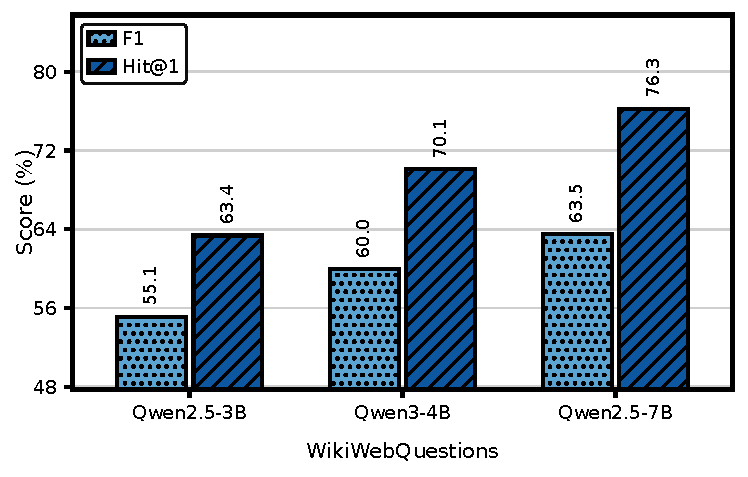
\includegraphics[width=0.32\textwidth]{figures/model_scale_sft_wikiwebquestions.pdf}\hfill
    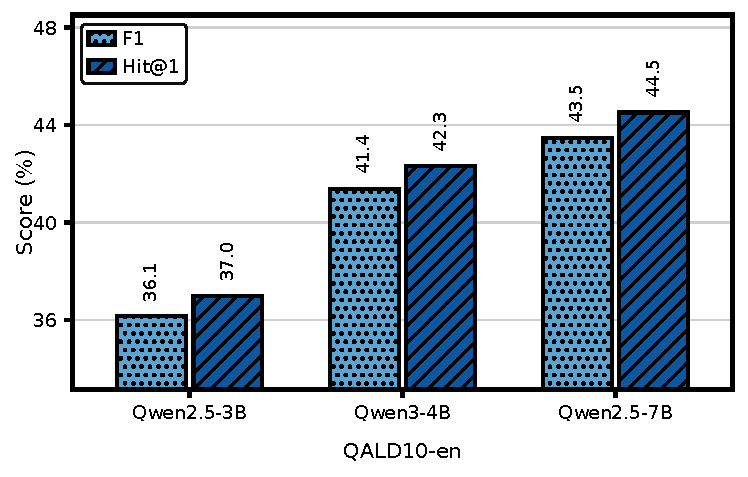
\includegraphics[width=0.32\textwidth]{figures/model_scale_sft_qald10en.pdf}\hfill
    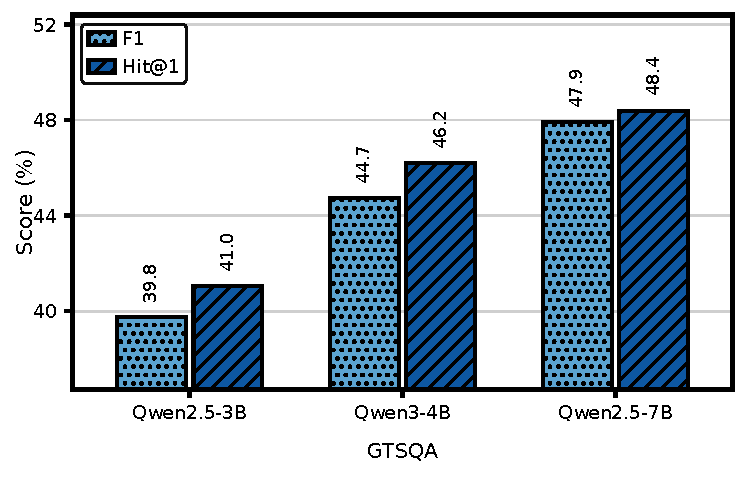
\includegraphics[width=0.32\textwidth]{figures/model_scale_sft_gtsqa.pdf}
    \caption{\textbf{Effect of model scale.} F1 and Hit@1 of backbones of different sizes after SFT on the same data.}
    \label{fig:model_scale}
    \vspace{-5mm}
\end{figure*}

As shown in Table~\ref{tab:rq4_ecpr_ablation}, we ablate the training stages and reward terms on the two benchmarks with gold supporting triples, under the same backbone, SFT checkpoint, RL data, and rollout budget, so the variants differ only in the reward.

\paragraph{Impact of RL.}
Full FoG improves over SFT only by +6.83 and +4.33 Hit@1, but RL without $R_{\text{ecpr}}$ raises Cov by only +2.28 and +1.58. This is because the outcome reward is paid in full once the answer is reached, whatever evidence is retrieved.

\paragraph{Impact of $R_{\text{ecpr}}$.}
Removing $R_{\text{ecpr}}$ causes the largest drop among the reward terms, and Cov drops more (5.43 and 7.21) than Hit@1 (2.58 and 3.55). As both variants share the data and the SFT checkpoint, this confirms that the coverage gain comes from the reward itself.

\paragraph{Impact of $R_{\text{step}}$.}
Removing $R_{\text{step}}$ lowers Hit@1 by 0.45 and 2.35 but Cov by only 1.09 and 1.43, indicating that step validity keeps the interaction executable but does not drive coverage.

\paragraph{ECPR vs.\ LLM-as-judge.}
An LLM-as-judge score of the reasoning process~\citep{KG-Hopper} raises Cov by only 1.21 and 1.93 over no process supervision and stays 4.22 and 5.28 below ECPR. This suggests that judging how plausible the reasoning reads is a weaker signal than ECPR.

\subsection{Evidence-Grounded Synthesis (RQ3)}
\label{sec:rq3}

As shown in Table~\ref{tab:rq3_synth_data} and Figure~\ref{fig:model_scale}, we fix a budget of 6,588 SFT questions and vary the data source (Train-Only, Synth-Only, or a mix of both), and apply the same SFT data to three backbone scales.

\paragraph{Validity of embedded evidence.}
The supporting triples of every retained question reproduce its answer under SPARQL execution, and the redundancy check misses a shortcut in only 1.5\% of 200 audited questions. This confirms that the embedded triples are a valid reward target without annotation.

\begin{table}[t]
\centering
\footnotesize
\setlength{\tabcolsep}{6pt}
\renewcommand{\arraystretch}{1.1}
\resizebox{\columnwidth}{!}{
\begin{tabular}{l|cc|cc|cc}
    \toprule
    \multirow{2}{*}{Data Source}
    & \multicolumn{2}{c|}{WikiWebQuestions}
    & \multicolumn{2}{c|}{QALD10-en}
    & \multicolumn{2}{c}{GTSQA} \\
    \cmidrule(l){2-7}
   & F1 & Hit@1 & F1 & Hit@1 & F1 & Hit@1 \\
    \midrule
    Train-Only
    & 53.58 & 64.51 & 36.94 & 37.86 & 41.33 & 41.52 \\
    Synth-Only
    & 57.84 & 68.17 & 39.52 & 40.36 & 43.21 & 44.58 \\
    \rowcolor{lightblue}
    \textbf{Mixed}
    & \best{59.95} & \best{70.10} & \best{41.38} & \best{42.31} & \best{44.73} & \best{46.19} \\
    \bottomrule
\end{tabular}}
\caption{\textbf{Impact of synthetic training data.}}
\label{tab:rq3_synth_data}
\end{table}

\begin{table}[!t]
\centering
\renewcommand{\arraystretch}{0.9}
\resizebox{\columnwidth}{!}{          
\begin{tabular}{l|ccc|ccc}
    \toprule
    \multirow{2}{*}{Methods} 
    & \multicolumn{3}{c|}{WikiWebQuestions} 
    & \multicolumn{3}{c}{GTSQA} \\ 
    \cmidrule(l){2-7} 
    & Hit@1 & RetQ & Cov
    & Hit@1 & RetQ & Cov \\ 
    \midrule
    PoG                        
    & 71.89 & 75.66 & 69.85 & 39.33 & 35.70 & 25.38 \\
    ToG                        
    & 72.75 & 73.53 & 68.79 & 42.36 & 50.99 & 37.34 \\
    KG-R1
    & 73.01 & 82.28 & 74.50 & 47.73 & 61.41 & 54.05 \\
        \rowcolor{lightblue}
    FoG-4B
    & \textbf{76.93} & \textbf{86.35} & \textbf{78.34} & \textbf{50.52} & \textbf{65.34} & \textbf{58.64} \\
    \bottomrule
\end{tabular}
}
\caption{\textbf{Answer accuracy and evidence coverage of agent-based methods.}}
\label{tab:rq2_faithful}
\end{table}

\paragraph{Synthetic vs.\ original data.}
Synth-Only outperforms Train-Only by +3.66, +2.50, and +3.06 Hit@1 with no in-domain question, indicating that questions built by backward expansion transfer to human-written benchmarks. Mixed performs best, so the two sources are complementary (Appendix~\ref{app:synth_cost}).

\paragraph{Performance across model scales.}
Hit@1 improves steadily from 3B to 7B (+12.89, +7.52, and +7.36), indicating that the synthetic data is not backbone-specific.

\subsection{Analysis of KG Interaction Agent (RQ4)}
\label{sec:rq4}

As shown in Table~\ref{tab:rq2_faithful} and Figure~\ref{fig:complexity}, we examine how much evidence agent-based methods retrieve.

\paragraph{Answers without evidence.}
On GTSQA, PoG attains 39.33 Hit@1 but reaches the gold answer on only 35.70\% of questions, so at least 9.2\% of its correct answers never appear in any KG observation, and the RL-trained KG-R1 still leaves 45.95\% of the supporting triples unretrieved. Neither prompting nor outcome rewards thus make an agent use the KG as a source of evidence.

\paragraph{Evidence coverage.}
FoG attains the highest Cov and RetQ on both benchmarks (+3.84 and +4.59 Cov over KG-R1) together with the highest Hit@1, indicating that evidence coverage does not come at the cost of answer accuracy (Appendix~\ref{app:casestudy}).

\paragraph{Performance under structural complexity.}
FoG leads KG-R1 on all 10 groups and is the best method on 9. Its margin over KG-R1 grows from +1.4 Hit@1 on $(1)$ to +5.0 on $(3)$ and +6.0 on the more branched $(3)(1)$, questions that depend on more supporting triples. This suggests that the more evidence an answer requires, the more the agent benefits from rewards for retrieving it, although the margin narrows to +2.0 on $(4)$.

\begin{figure*}[t]
    \centering
    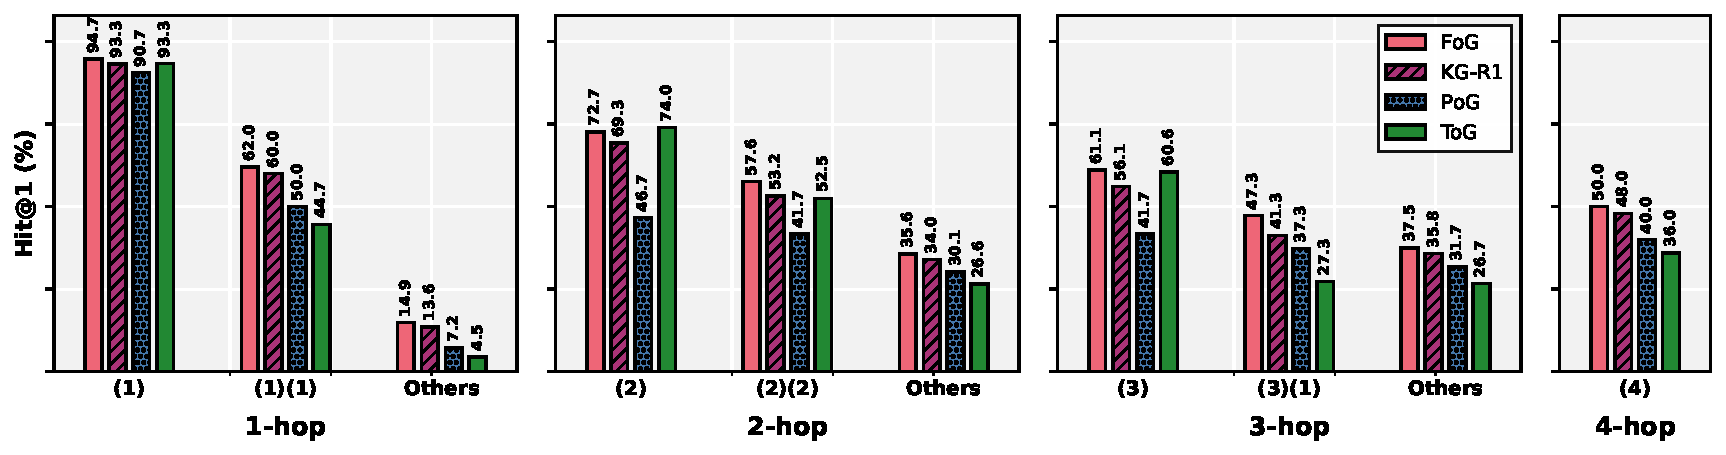
\includegraphics[width=\linewidth]{figures/complex_reasoning.pdf}
    \caption{\textbf{Performance under structural complexity on GTSQA} by reasoning hop and isomorphism type.}
    \label{fig:complexity}
    \vspace{-5mm}
\end{figure*}
\begin{figure*}[t]
    \centering
    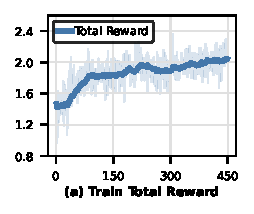
\includegraphics[width=0.245\textwidth]{figures/training_dynamics_reward.pdf}\hfill
    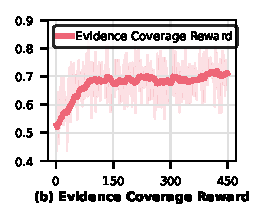
\includegraphics[width=0.245\textwidth]{figures/training_dynamics_coverage.pdf}\hfill
    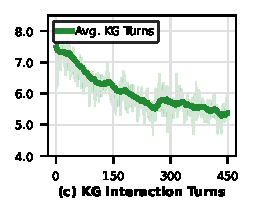
\includegraphics[width=0.245\textwidth]{figures/training_dynamics_turns.pdf}\hfill
    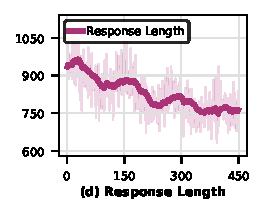
\includegraphics[width=0.245\textwidth]{figures/training_dynamics_length.pdf}
    \caption{\textbf{Training dynamics of FoG.} Rewards rise while interaction turns and response length decline.}
    \label{fig:training_dynamics}
    \vspace{-5mm}
\end{figure*}

\subsection{Analysis of ECPR (RQ5)}
\label{sec:rq5}
\begin{table}[t]
\centering
\small
\begin{tabular}{lccc}
\toprule
\textbf{Credit assignment} & \textbf{Hit@1} & \textbf{Cov} & \textbf{Dup.\ rate} \\
\midrule
Trajectory-level & 46.69 & 54.29 & 11.8\% \\
Every-match      & 47.01 & 52.21 & 29.4\% \\
\rowcolor{lightblue}
\textbf{First-match (ours)} & 50.52 & 58.64 & 8.6\% \\
\bottomrule
\end{tabular}
\caption{\textbf{Credit-assignment strategies for ECPR on GTSQA.} Dup.\ rate is the fraction of KG queries that re-retrieve an already retrieved gold triple.}
\label{tab:credit_assign}
\vspace{-5mm}
\end{table}


As shown in Table~\ref{tab:credit_assign} and Figure~\ref{fig:training_dynamics}, we compare first-match with \emph{trajectory-level} attribution, which credits coverage to the final turn, and \emph{every-match} attribution, which rewards every retrieval.

\paragraph{Comparison across attribution strategies.}
First-match achieves the best Hit@1 and Cov. Trajectory-level attribution loses 4.35 Cov, as turns that retrieve evidence earn the same return as the others. Every-match raises the duplicate-retrieval rate from 8.6\% to 29.4\% and falls below trajectory-level in Cov, as it rewards re-querying known evidence. This indicates that dense credit must pay each triple once, or it rewards redundant retrieval rather than coverage.

\paragraph{Training dynamics.}
Rewards rise during RL while KG turns and response length decline, indicating that the agent learns a precise retrieval policy that covers more evidence with fewer queries.

\begin{table}[t]
\centering
\footnotesize
\setlength{\tabcolsep}{5pt}
\renewcommand{\arraystretch}{1.1}
\resizebox{\columnwidth}{!}{
\begin{tabular}{l l l c c}
    \toprule
    \multirow{2}{*}{\textbf{Method}}
    & \multirow{2}{*}{\textbf{Train KG}}
    & \multirow{2}{*}{\textbf{Backbone}}
    & \textbf{WebQSP} & \textbf{WebQSP} \\
    & & & \textbf{train} & \textbf{Hit@1} \\
    \midrule
    ToG~\cite{ToG}          & None     & GPT-4                & No  & 82.6 \\
    RoG~\cite{RoG}          & Freebase & LLaMA2-Chat-7B       & Yes & 85.7 \\
    KG-R1~\cite{KG-R1}      & Freebase & Qwen2.5-3B-Instruct  & Yes & 82.8 \\
    \midrule
    FoG SFT-only            & Wikidata & Qwen3-4B-Instruct    & No  & 71.6 \\
    \textbf{FoG full}       & Wikidata & Qwen3-4B-Instruct    & No  & 77.2 \\
    \bottomrule
\end{tabular}}
\caption{\textbf{Zero-shot cross-KG transfer to Freebase (WebQSP).} Methods developed on Freebase are reference points, not matched baselines.}
\label{tab:rq5_crosskg}
\vspace{-5mm}
\end{table}

\subsection{Cross-KG Transfer (RQ6)}
\label{sec:rq6}

As shown in Table~\ref{tab:rq5_crosskg}, we evaluate the frozen FoG zero-shot on WebQSP over a Freebase backend.

\paragraph{Zero-shot transfer.}
FoG reaches 77.2 Hit@1 on an unseen KG, close to the methods developed on Freebase (82.6--85.7), and RL with ECPR contributes +5.6 Hit@1 over SFT only. This suggests that ECPR teaches the habit of retrieving evidence before answering, not the relations of one schema.
